% Appendix A

\chapter{Lithium Intercalation} % Main appendix title

%\label{AppendixA} % For referencing this appendix elsewhere, use \ref{AppendixA}

%\lhead{Appendix A. \emph{Appendix Title Here}} % This is for the header on each page - perhaps a shortened title

\begin{landscape}
\begin{figure}[!htp]
\centering
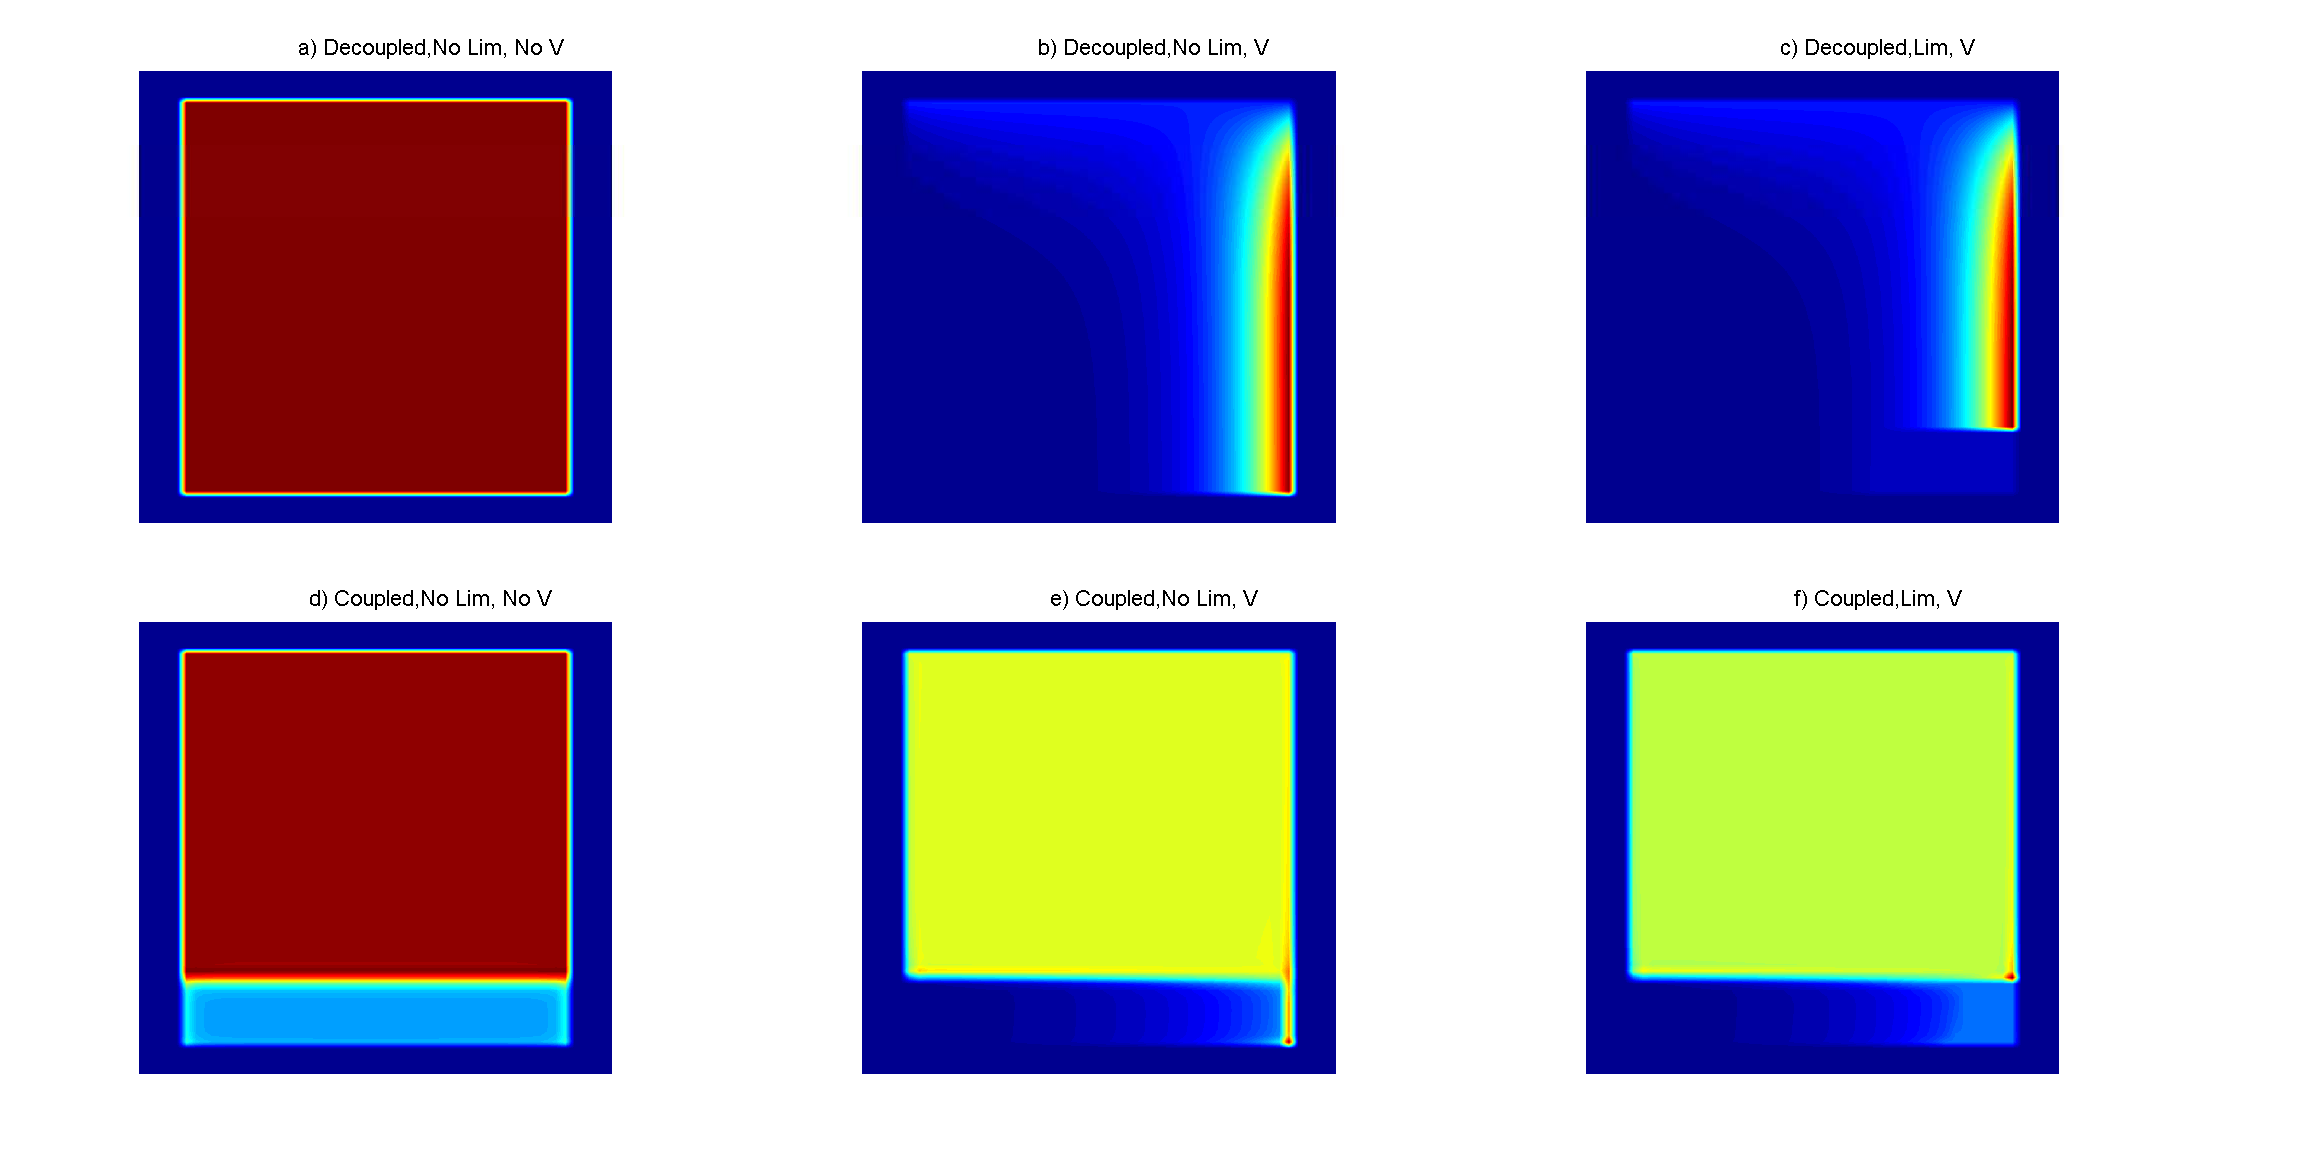
\includegraphics[scale=0.65]{Np61102}
\caption{Lithium Density in Steady State} 
\label{Np61102}
\end{figure}
\end{landscape}
 

\begin{landscape}
\begin{figure}[!htp]
\centering
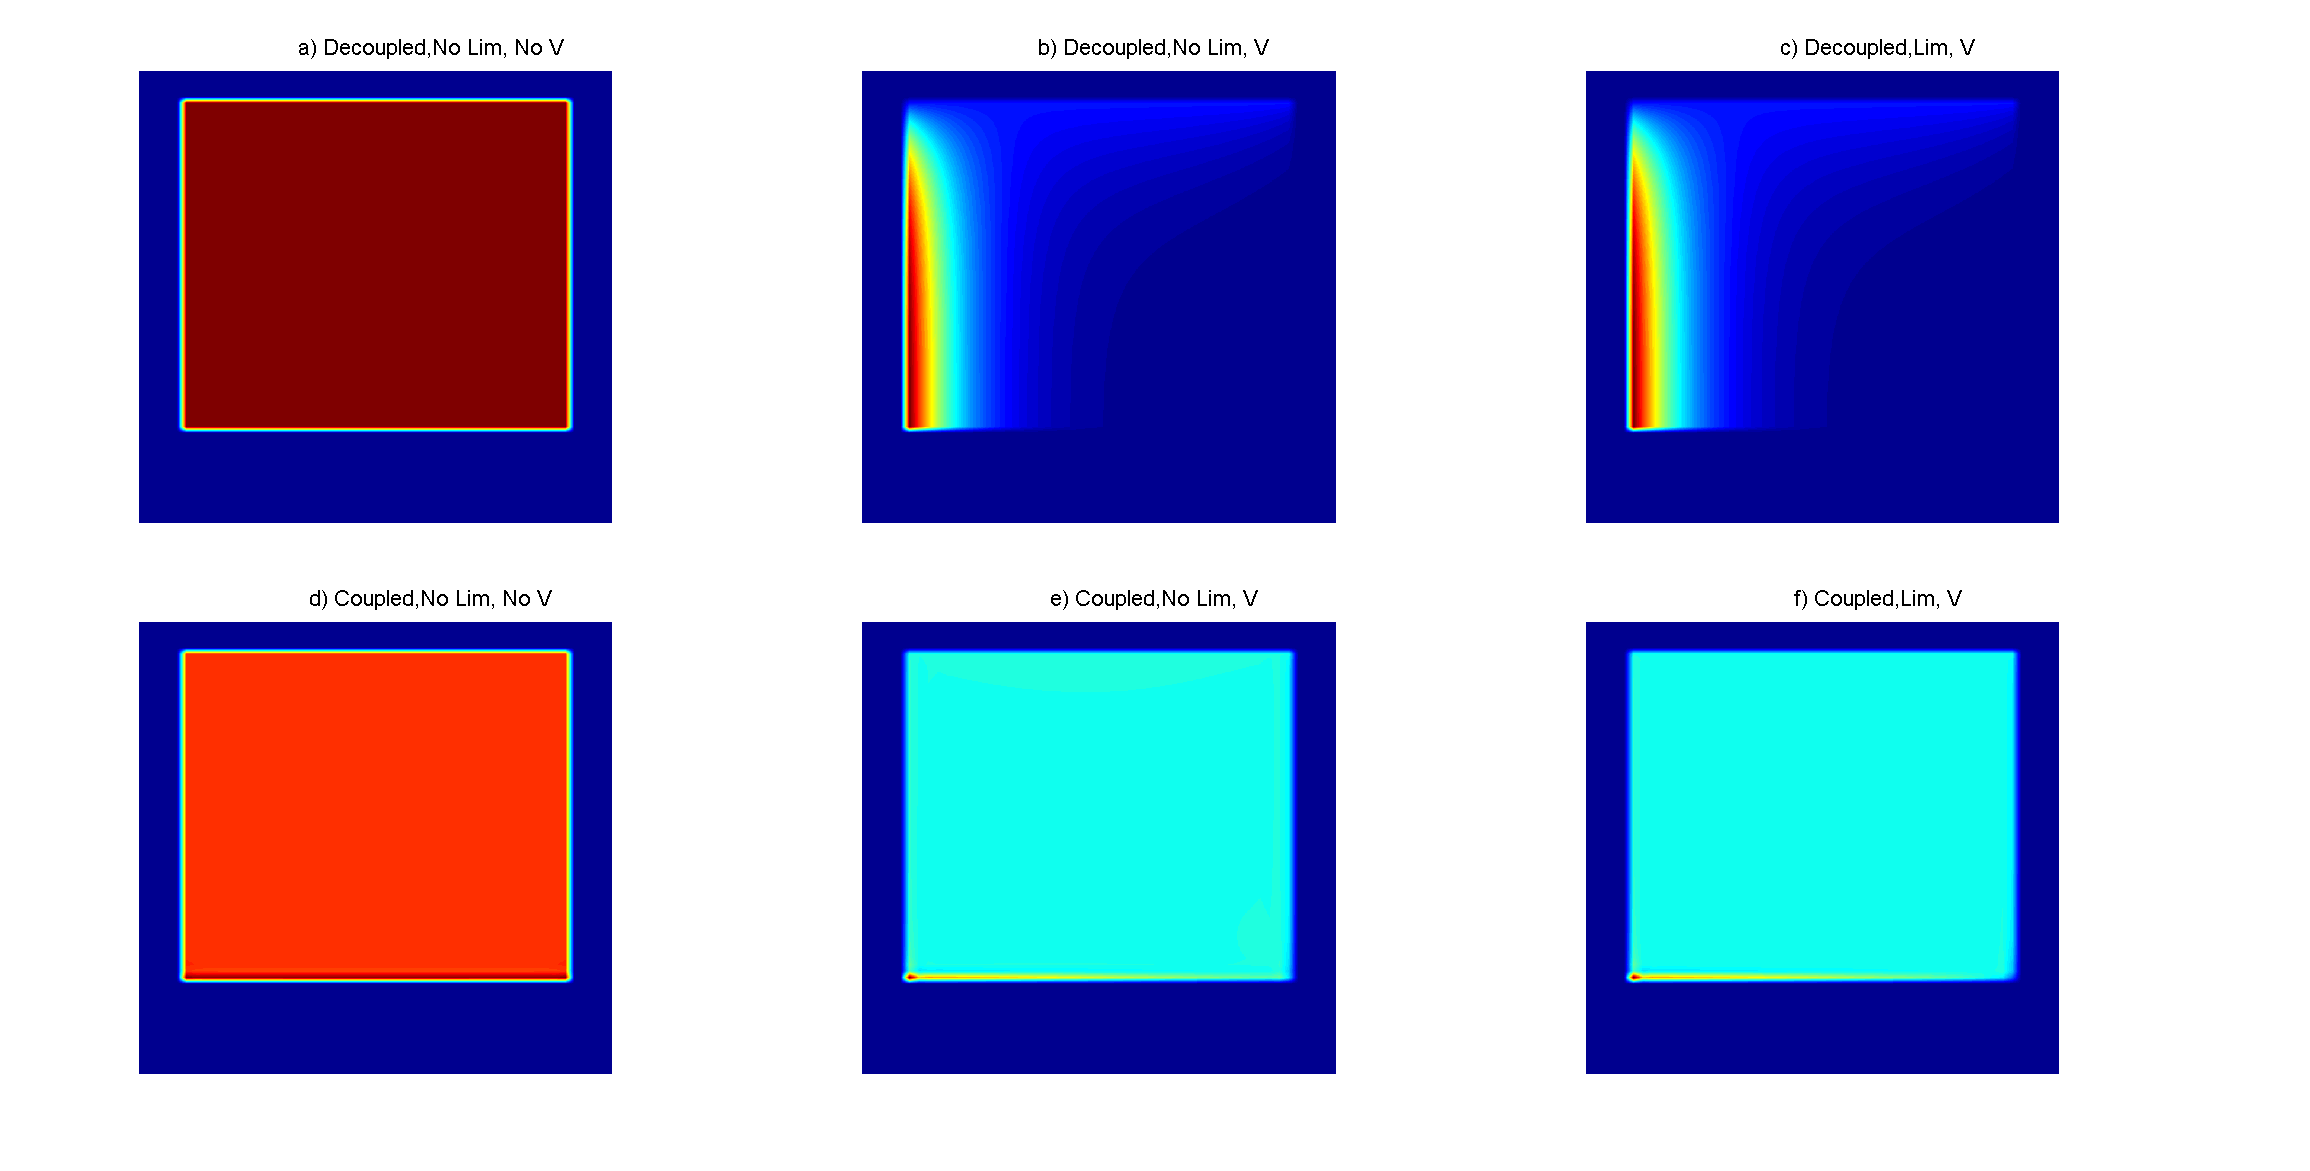
\includegraphics[scale=0.65]{Nn61102}
\caption{Cadmium Density in Steady State} 
\end{figure}
\end{landscape}


\begin{landscape}
\begin{figure}[!htp]
\centering
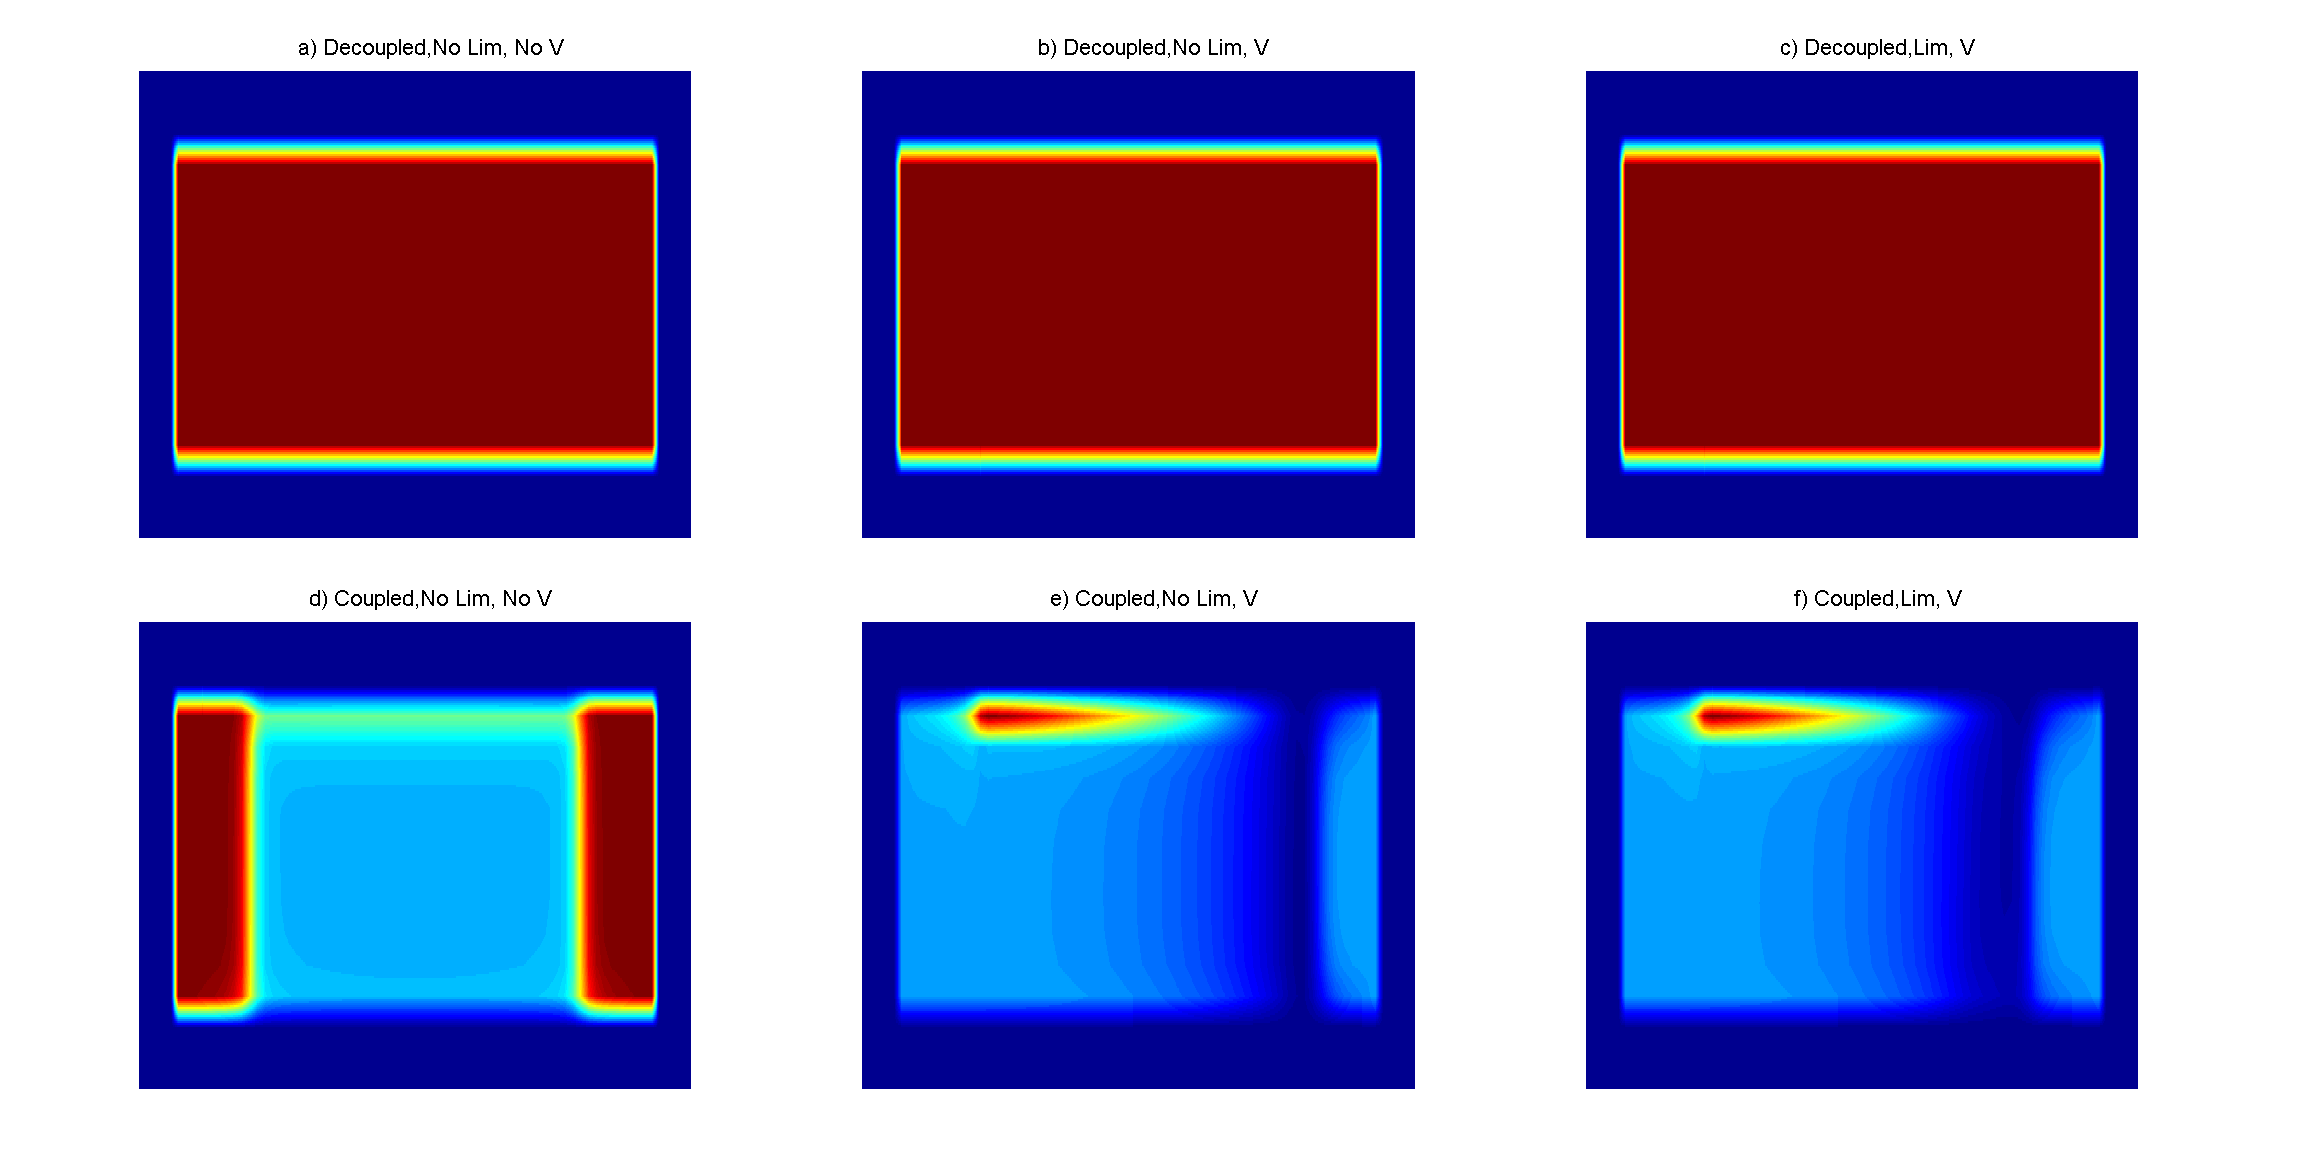
\includegraphics[scale=0.65]{p61102}
\caption{Hole Density in Steady State} 
\end{figure}
\end{landscape}

\begin{landscape}
\begin{figure}[!htp]
\centering
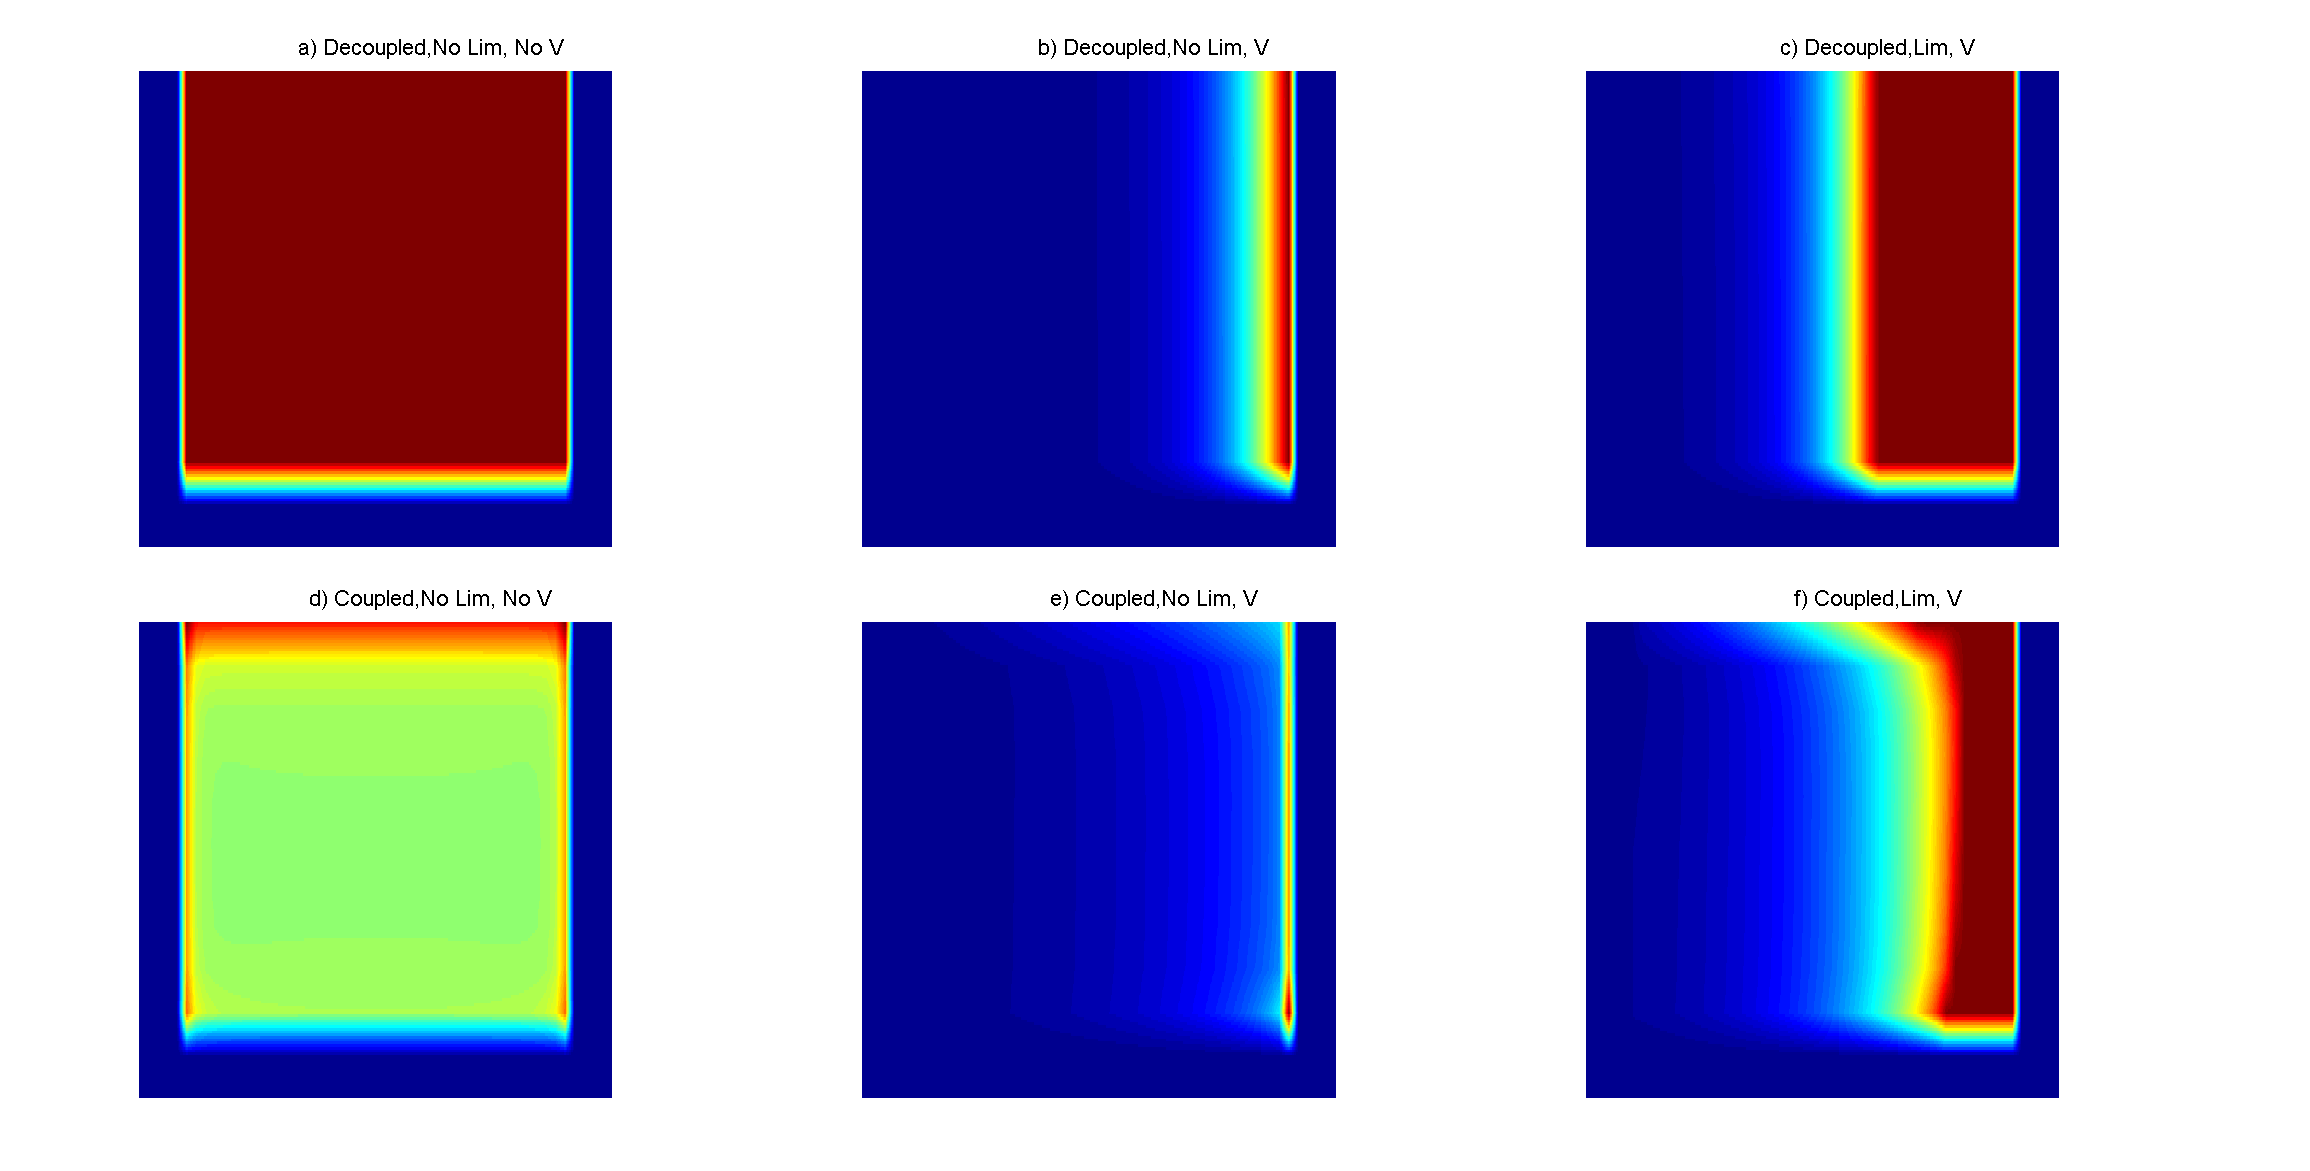
\includegraphics[scale=0.65]{Np61103}
\caption{2d Lithium Steady State PEDOT} 
\end{figure}
\end{landscape}

\begin{landscape}
\begin{figure}[!htp]
\centering
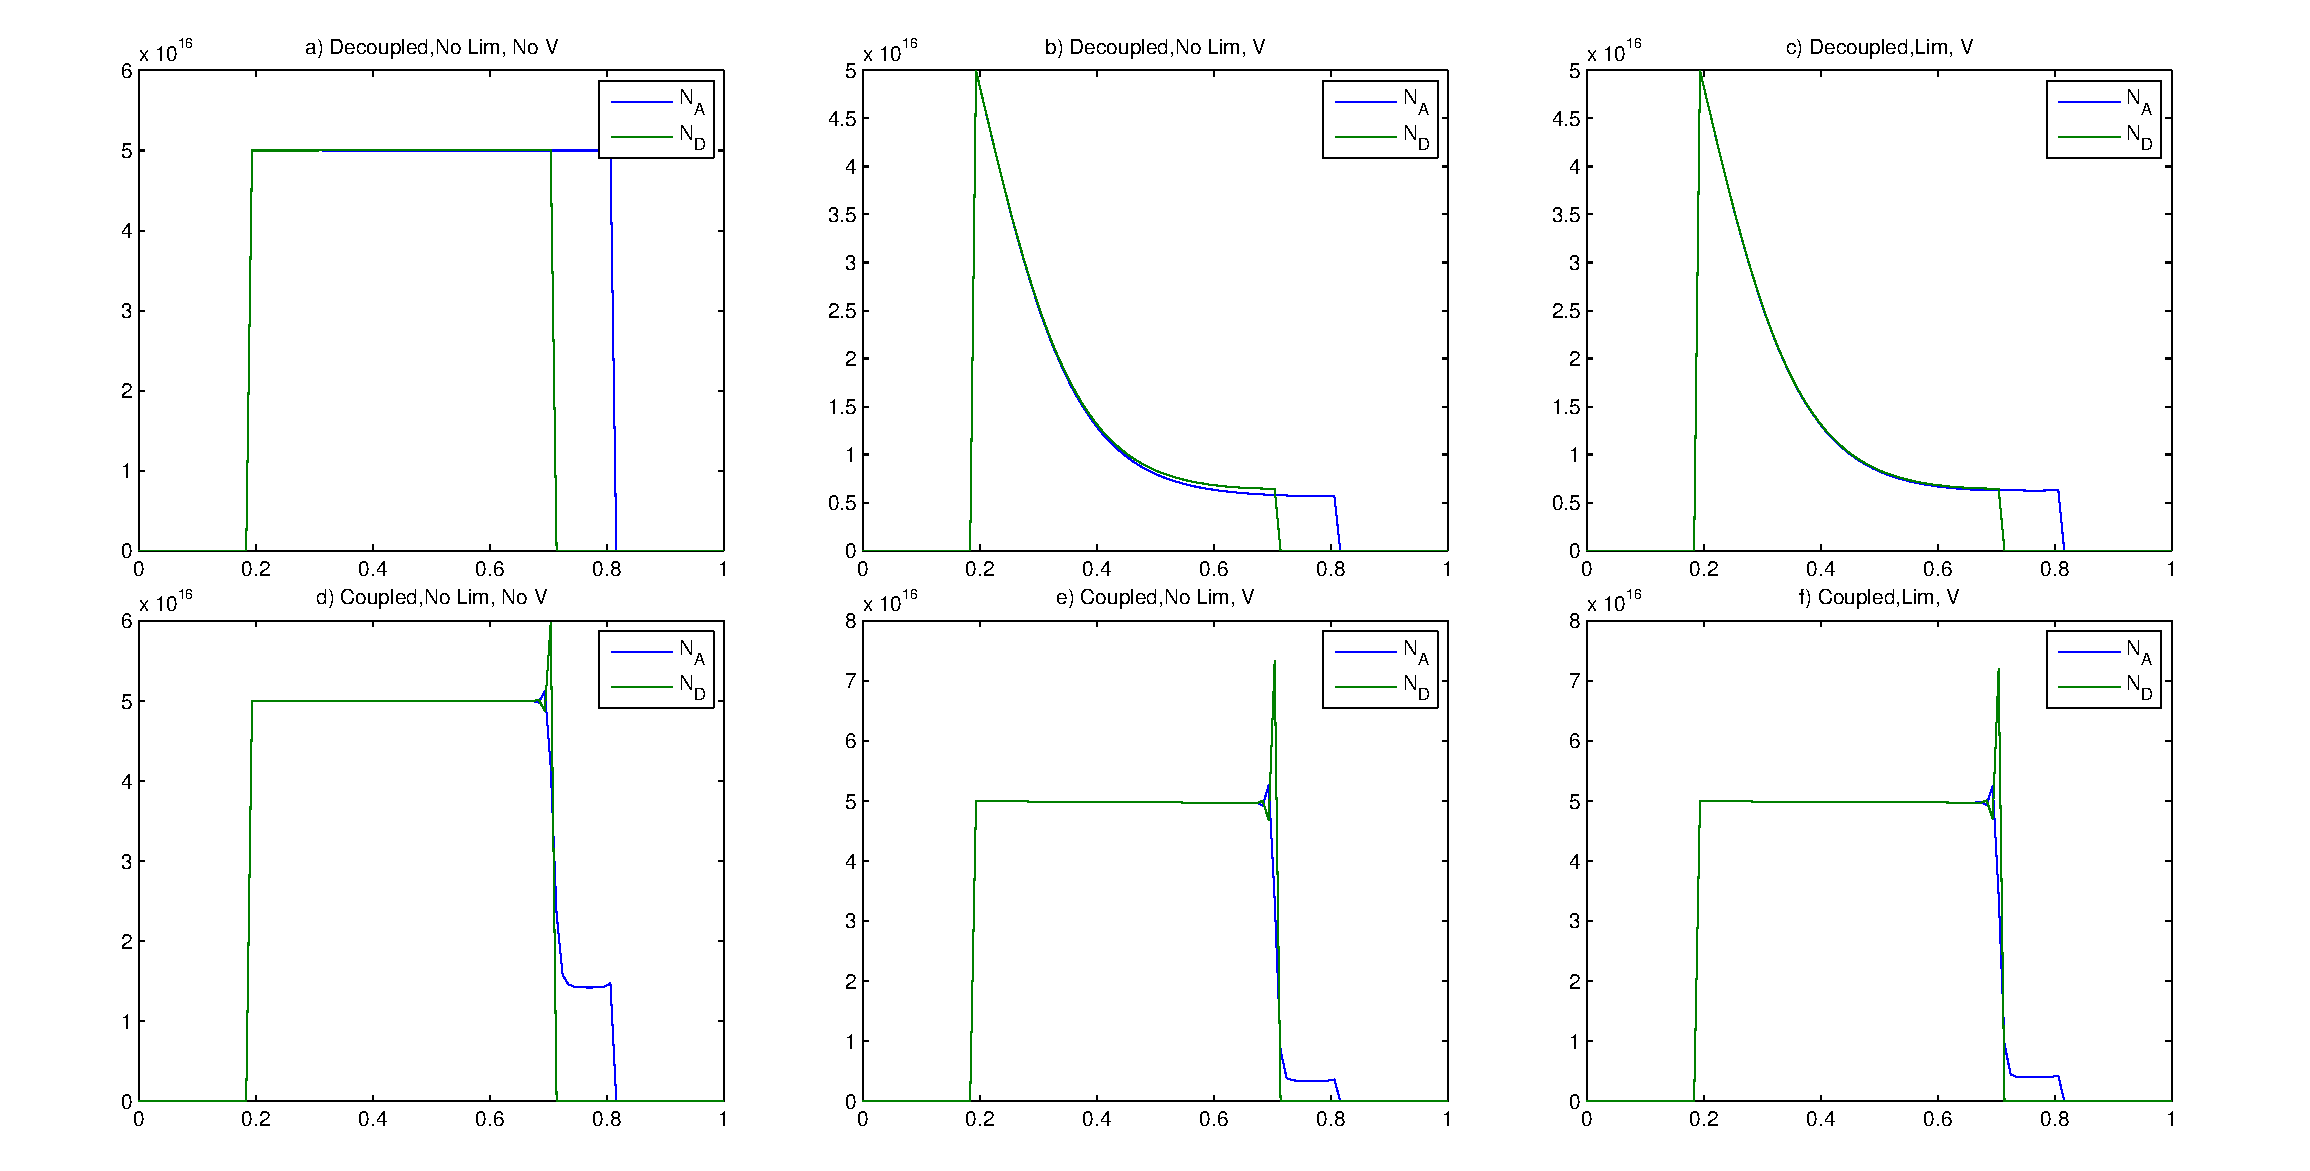
\includegraphics[scale=0.65]{NpNn61105}
\caption{1D Nn Lithium Vertical} 
\end{figure}
\end{landscape}

\begin{landscape}
\begin{figure}[!htp]
\centering
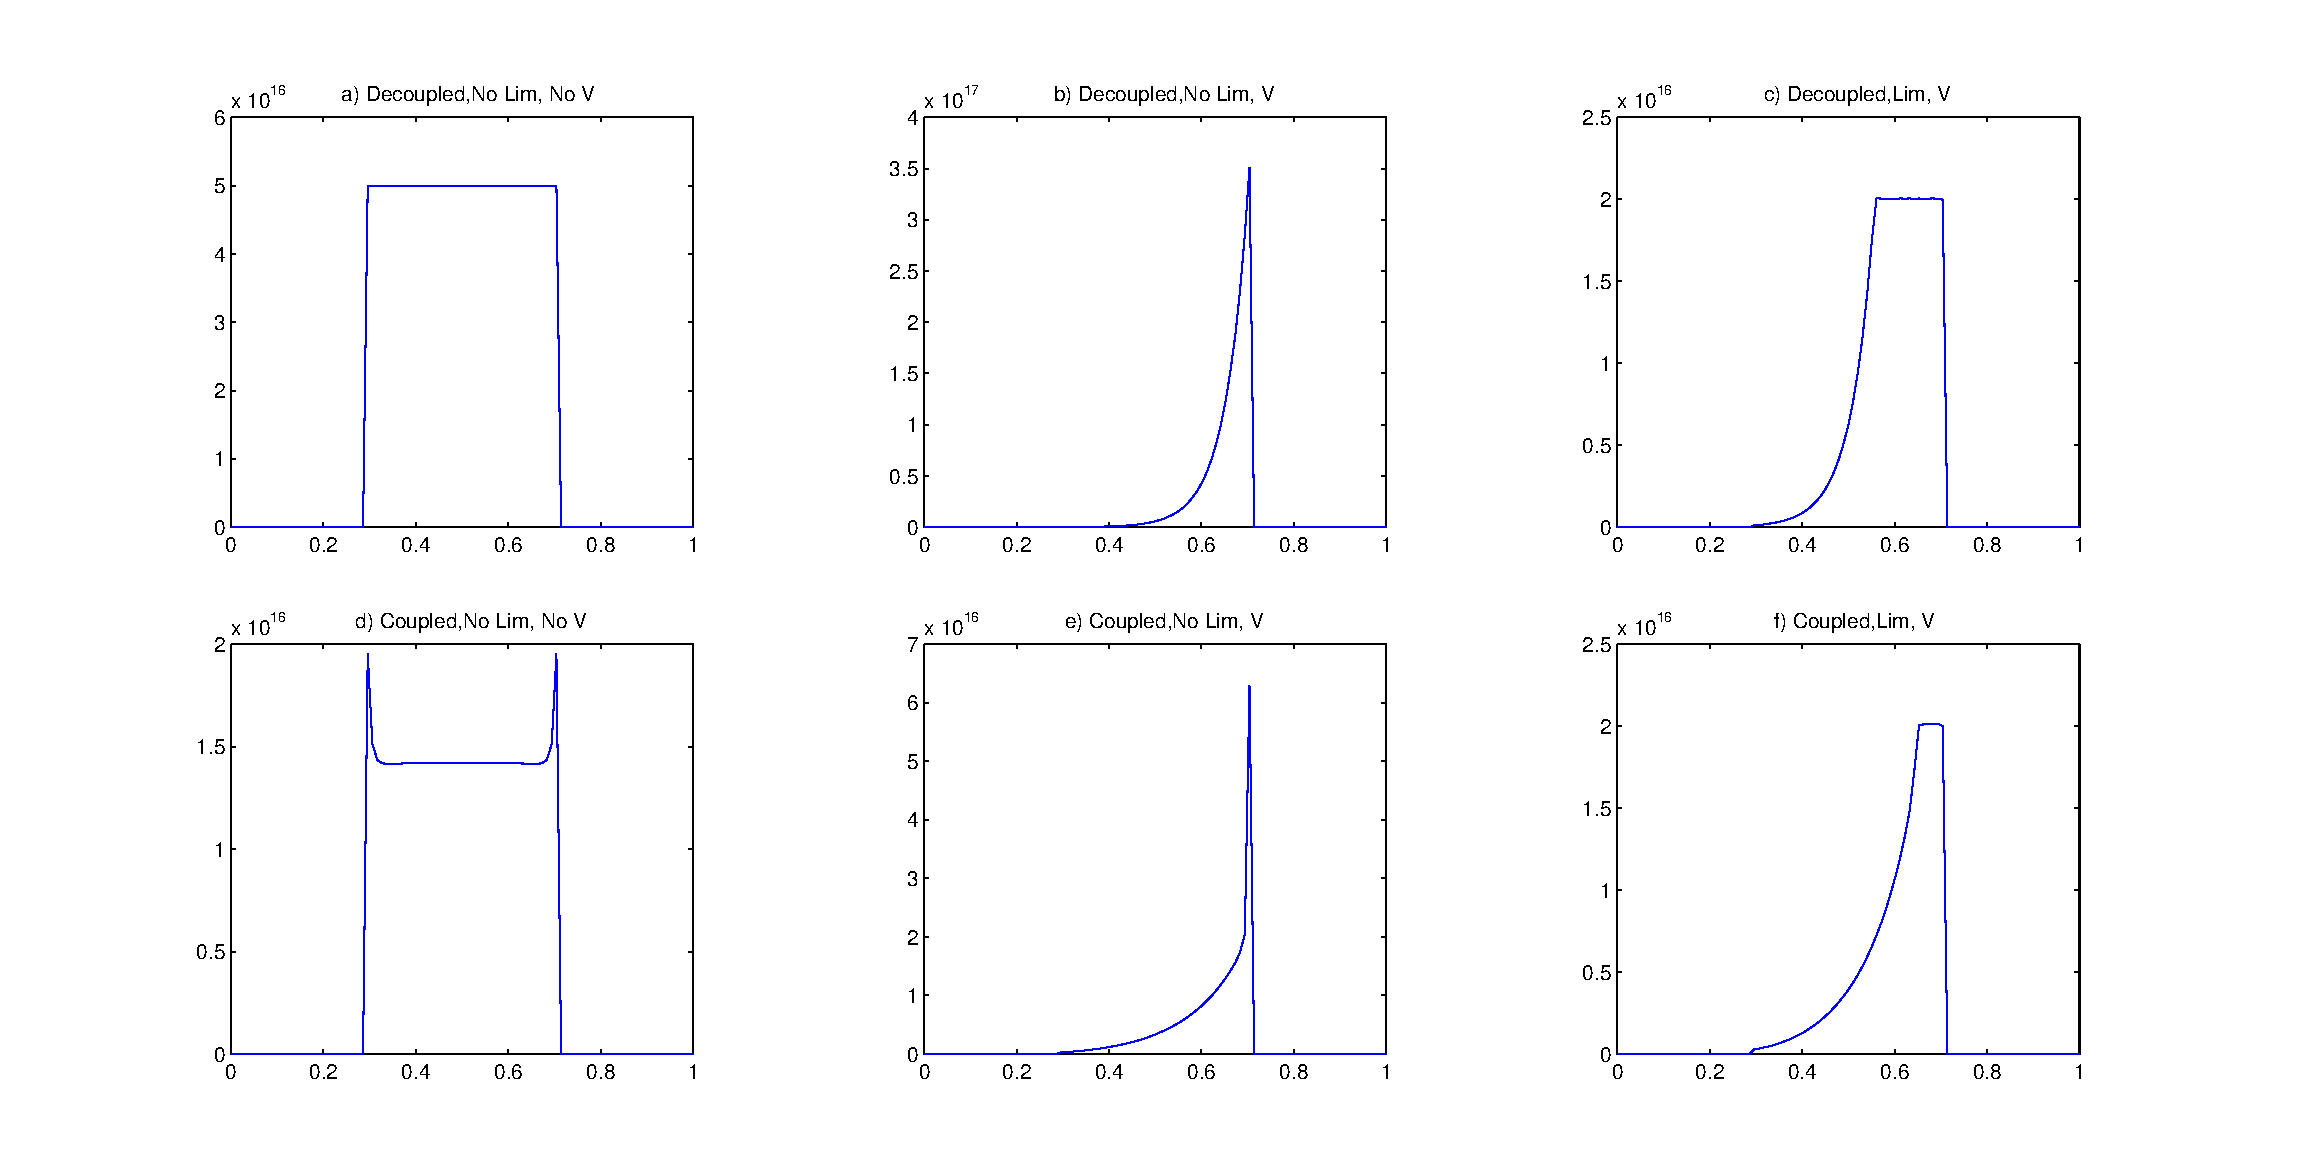
\includegraphics[scale=0.65]{Np61104}
\caption{1d Lithium Horizontal} 
\end{figure}
\end{landscape}

\begin{landscape}
\begin{figure}[!htp]
\centering
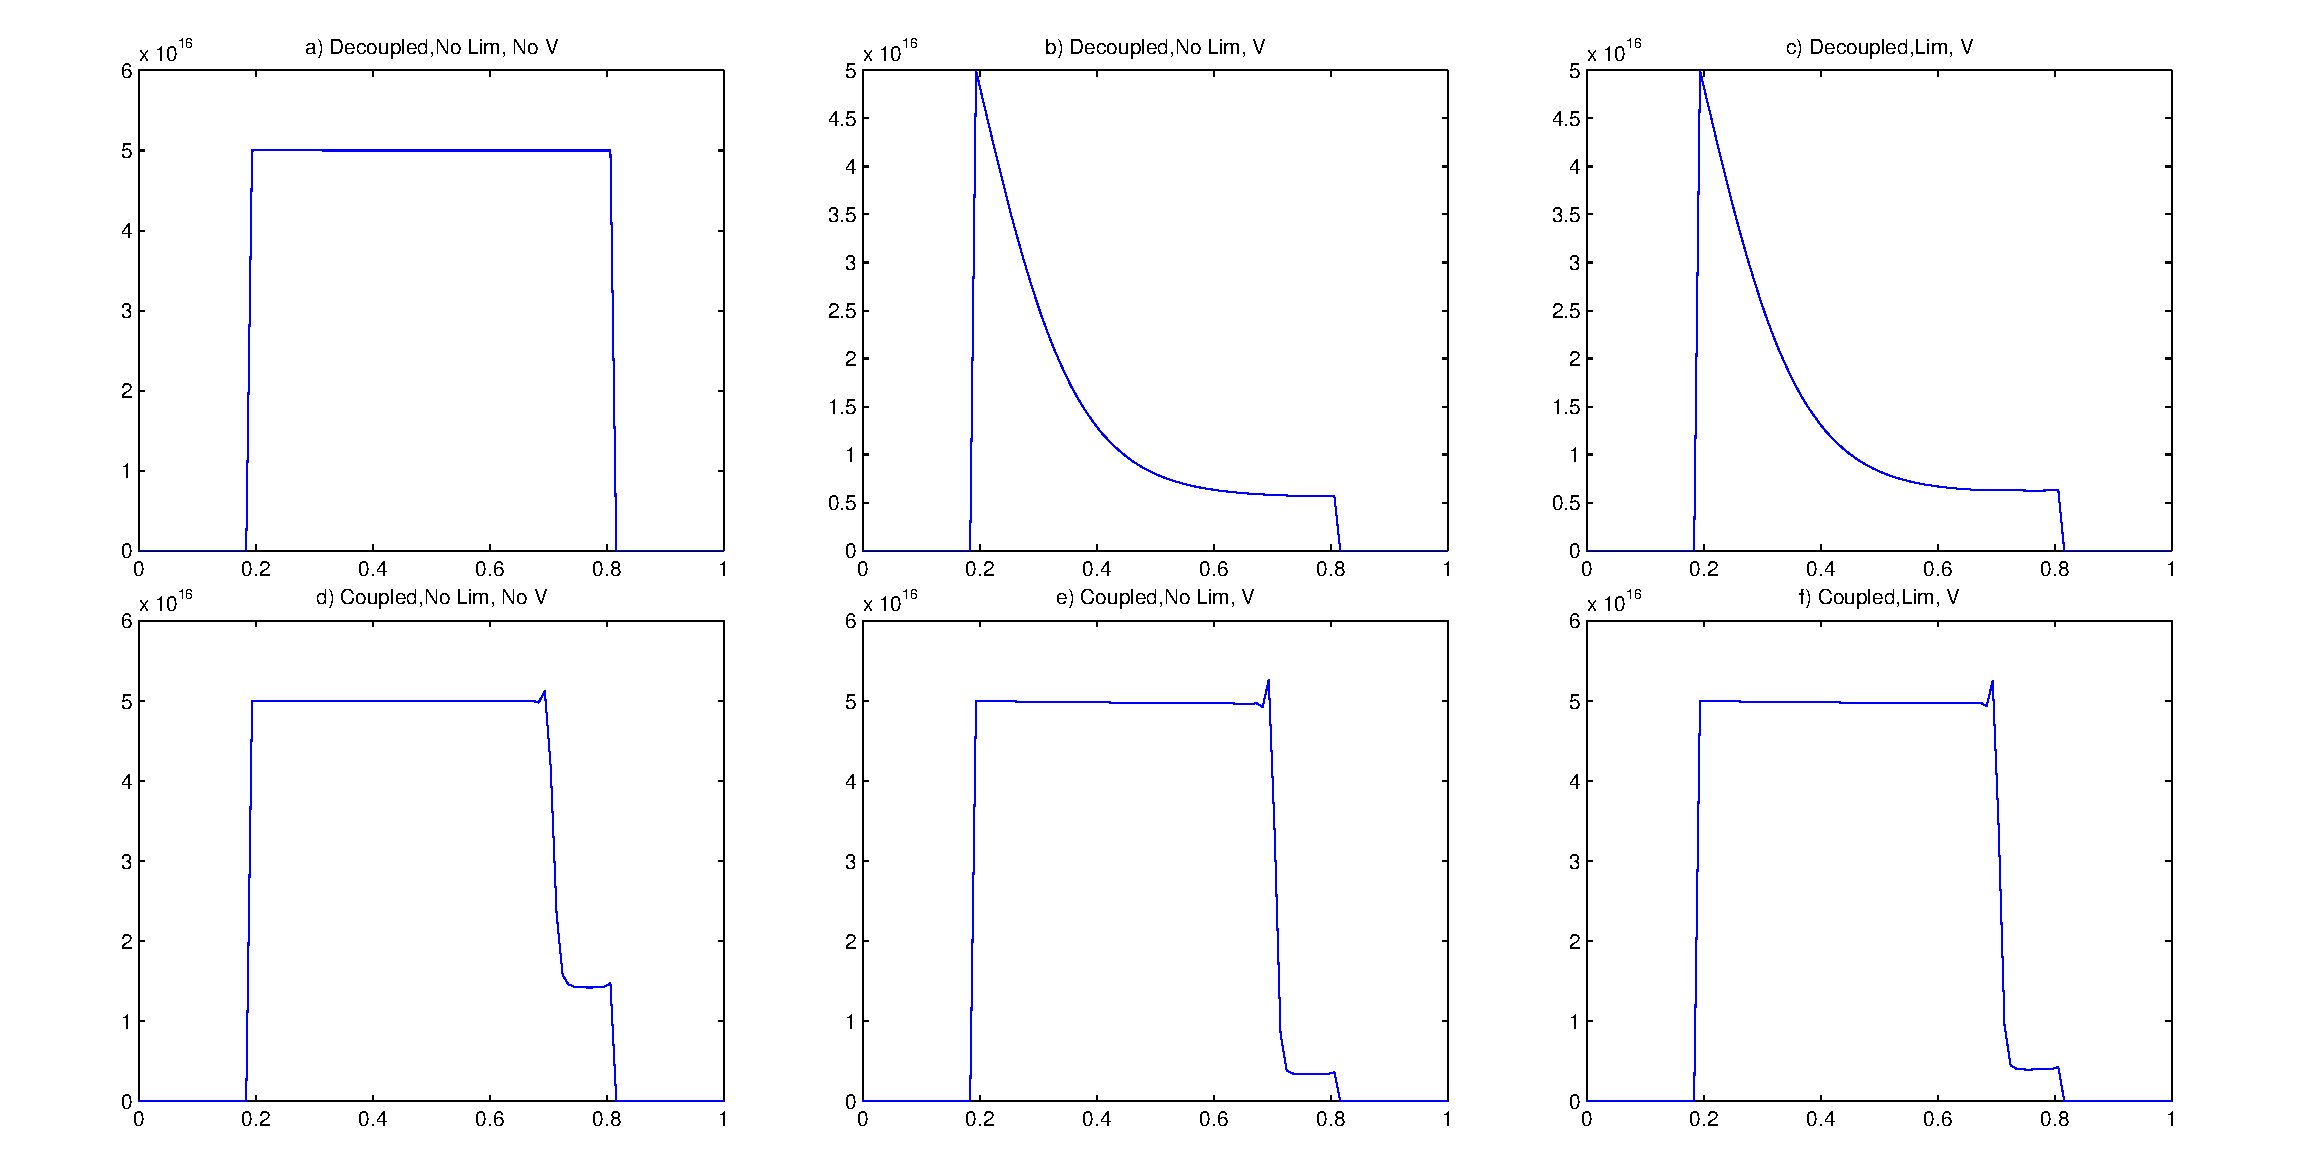
\includegraphics[scale=0.65]{Np61105}
\caption{1d Lithium Vertical} 
\end{figure}
\end{landscape}


\begin{landscape}
\begin{figure}[!htp]
\centering
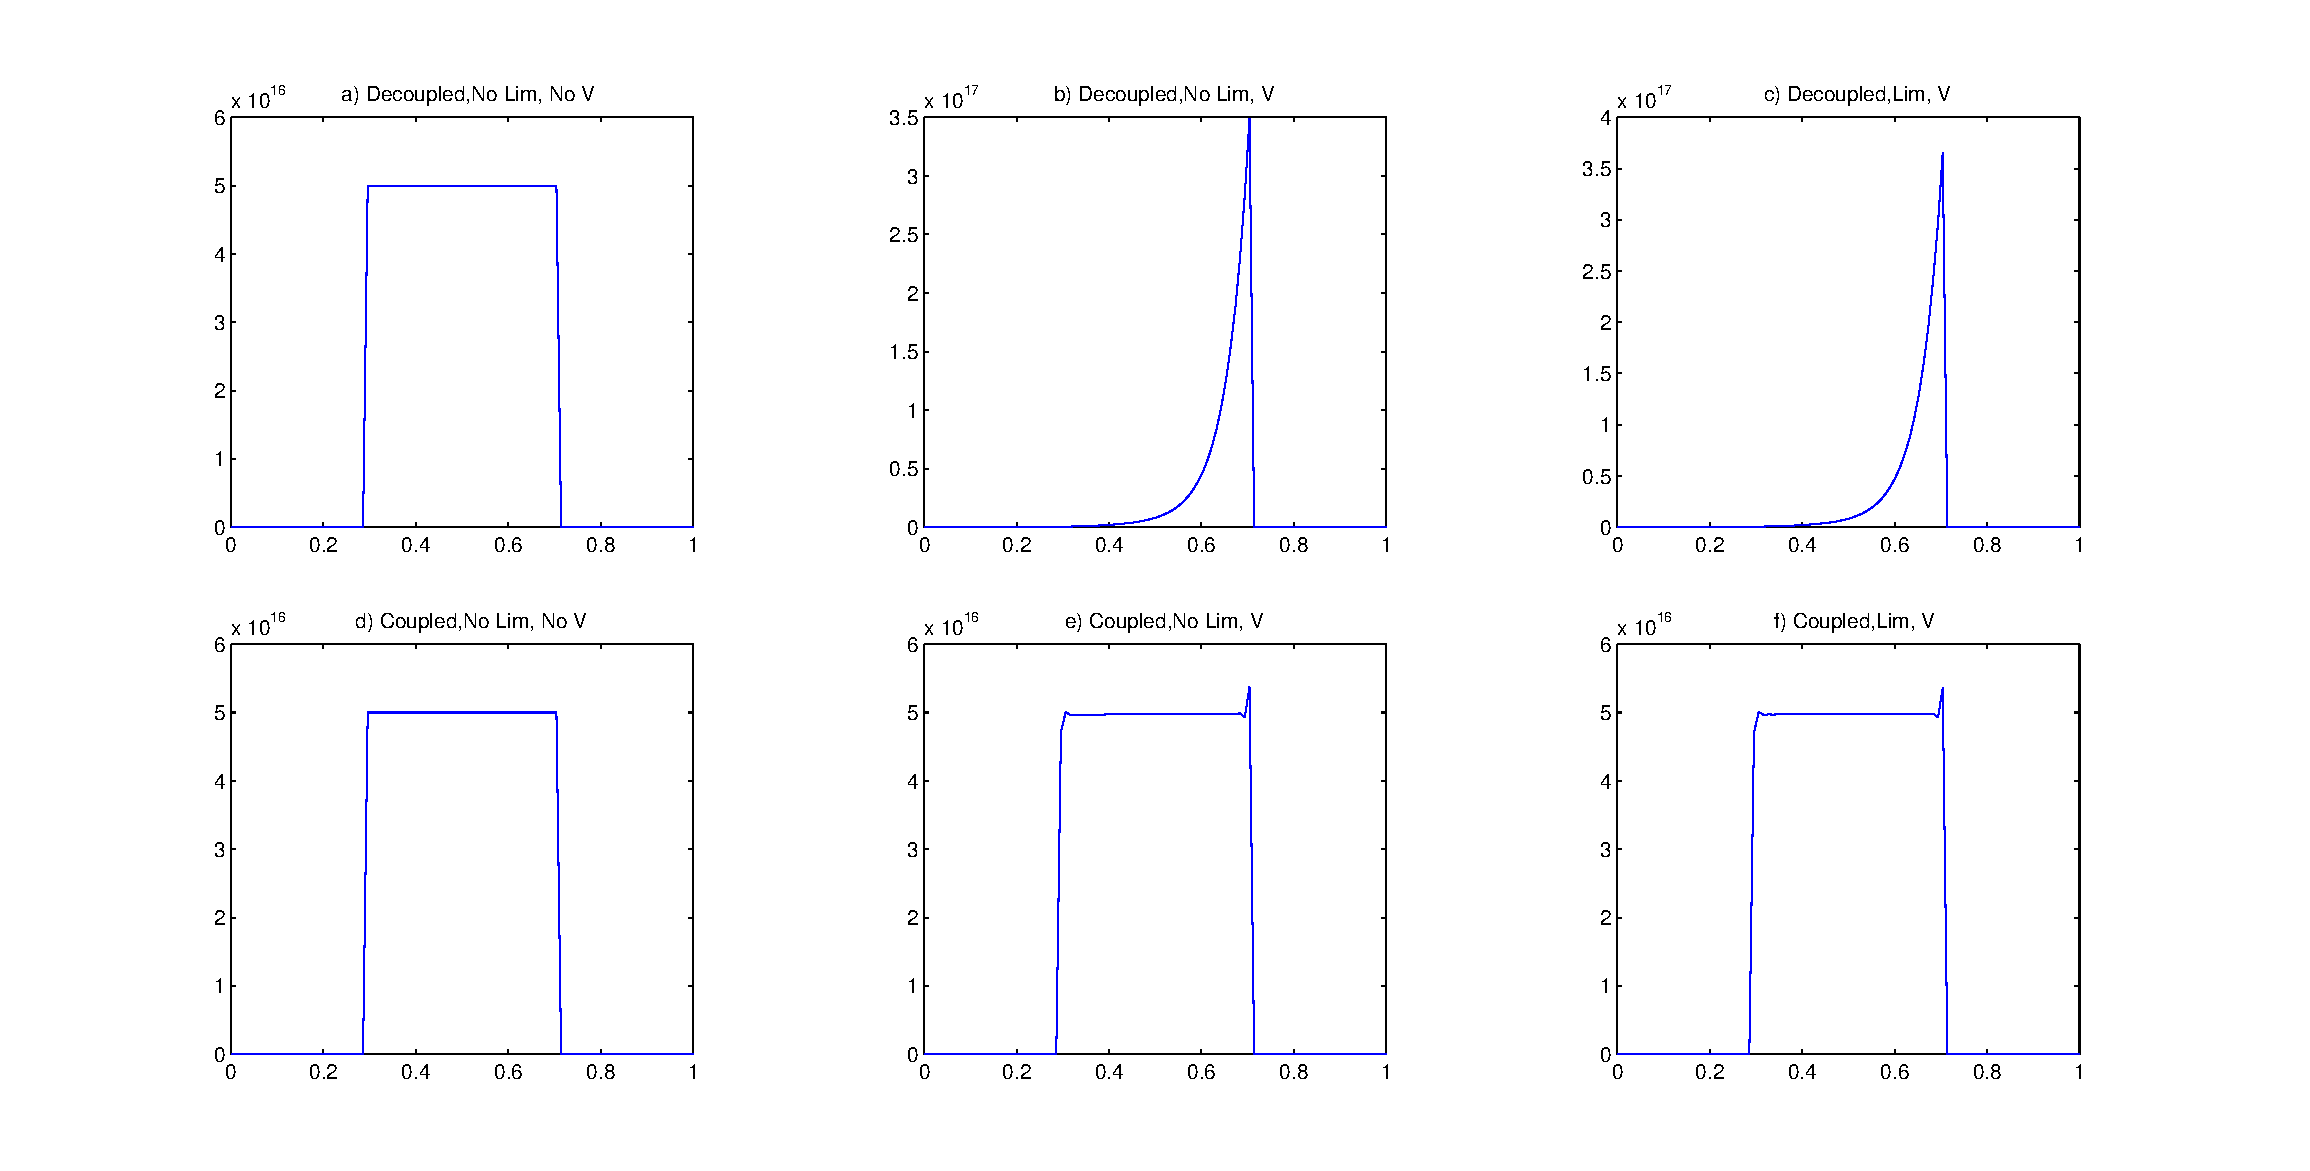
\includegraphics[scale=0.65]{Nn61104}
\caption{1D Nn Horizontal} 
\end{figure}
\end{landscape}

\begin{landscape}
\begin{figure}[!htp]
\centering
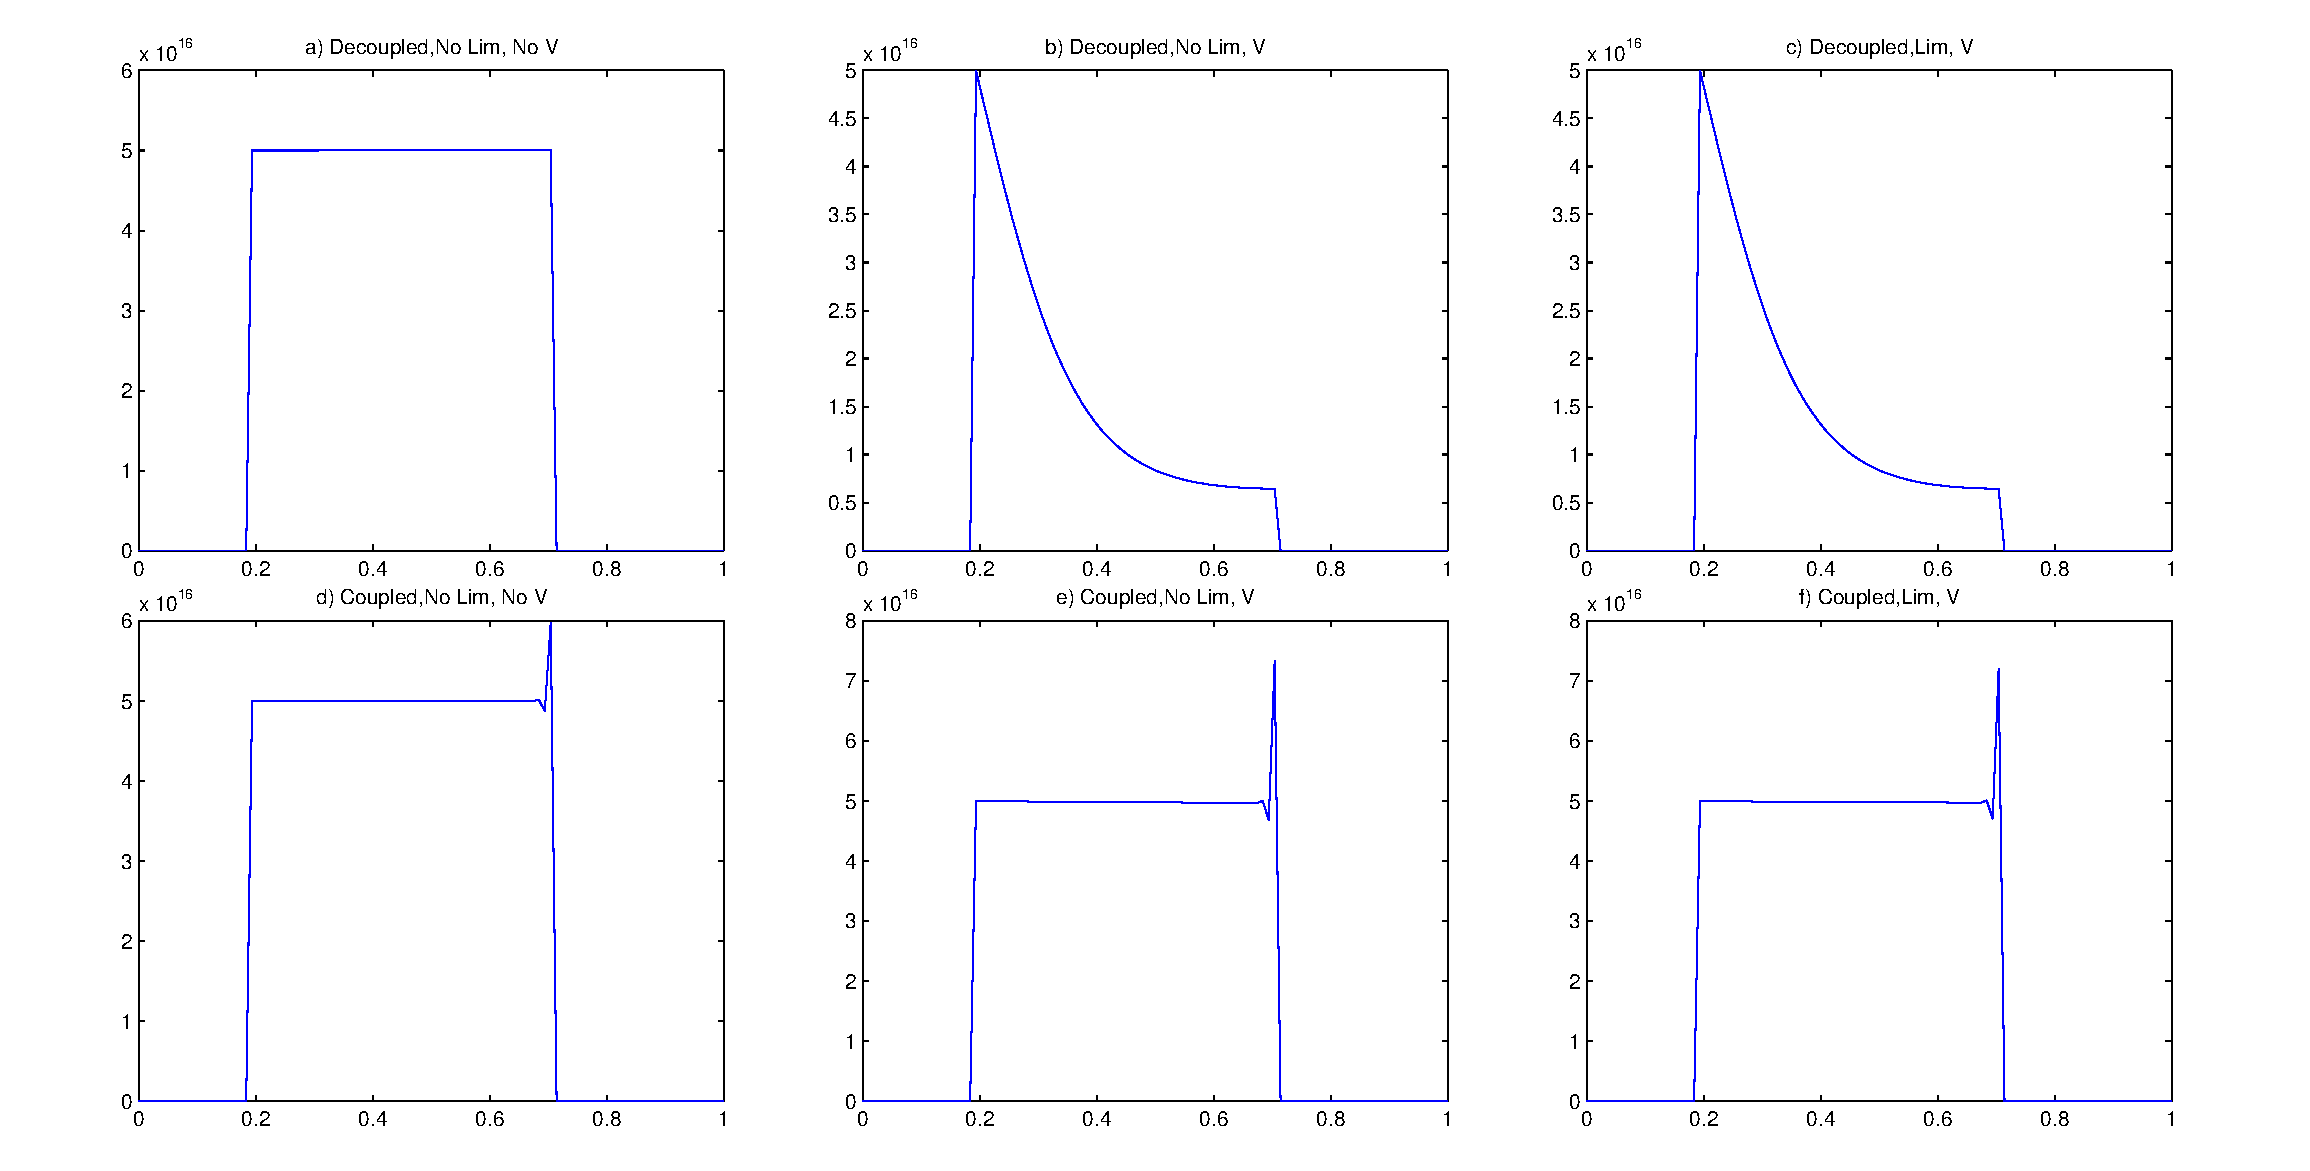
\includegraphics[scale=0.65]{Nn61105}
\caption{1D Nn Vertical} 
\end{figure}
\end{landscape}

\begin{landscape}
\begin{figure}[!htp]
\centering
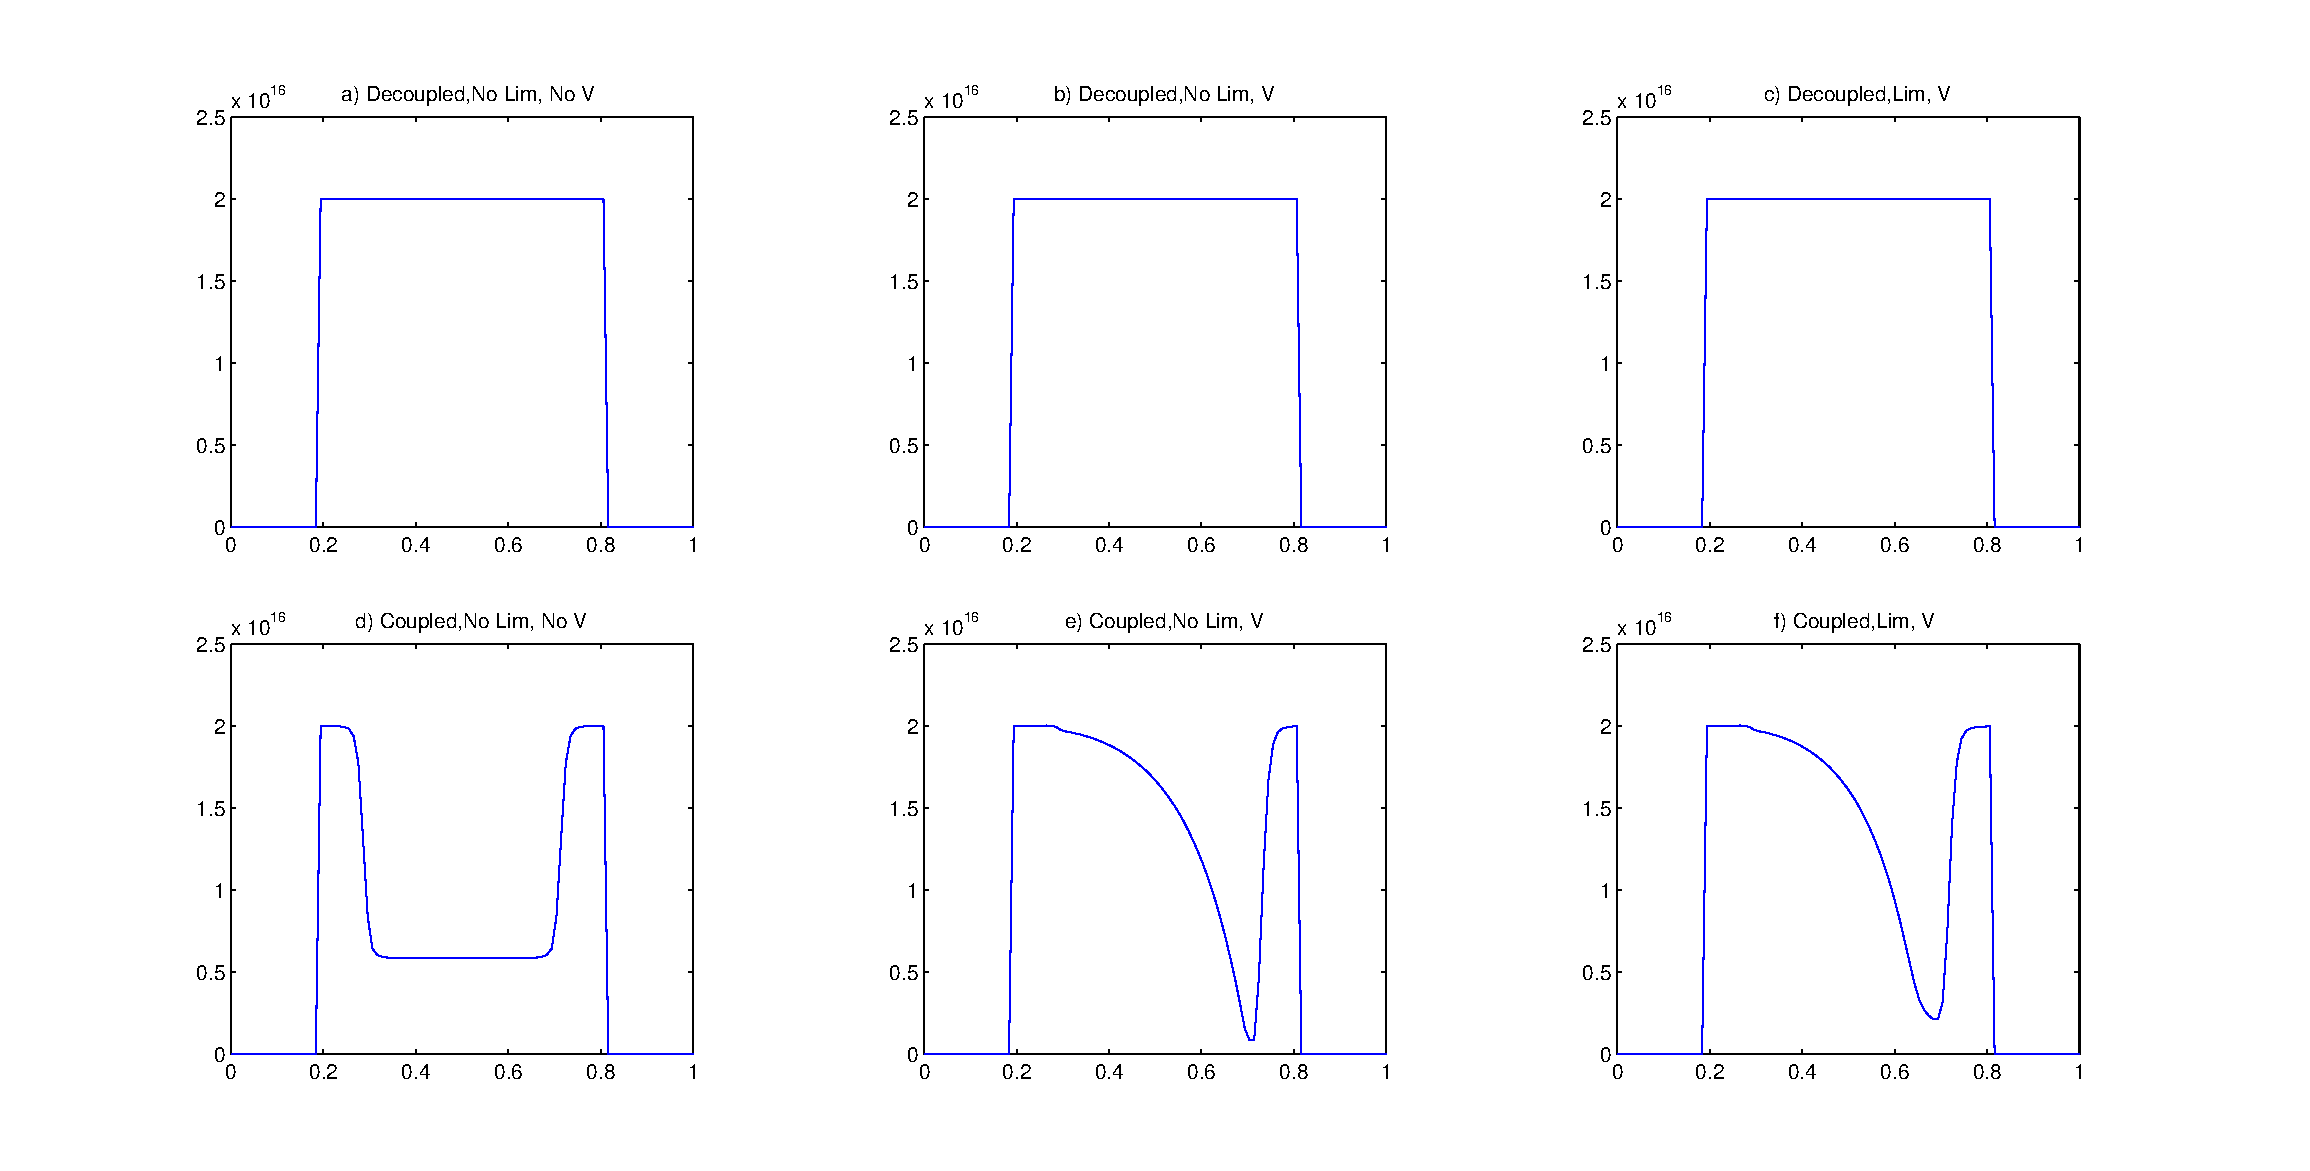
\includegraphics[scale=0.65]{p61104}
\caption{1-D Holes Vertical} 
\end{figure}
\end{landscape}

\begin{landscape}
\begin{figure}[!htp]
\centering
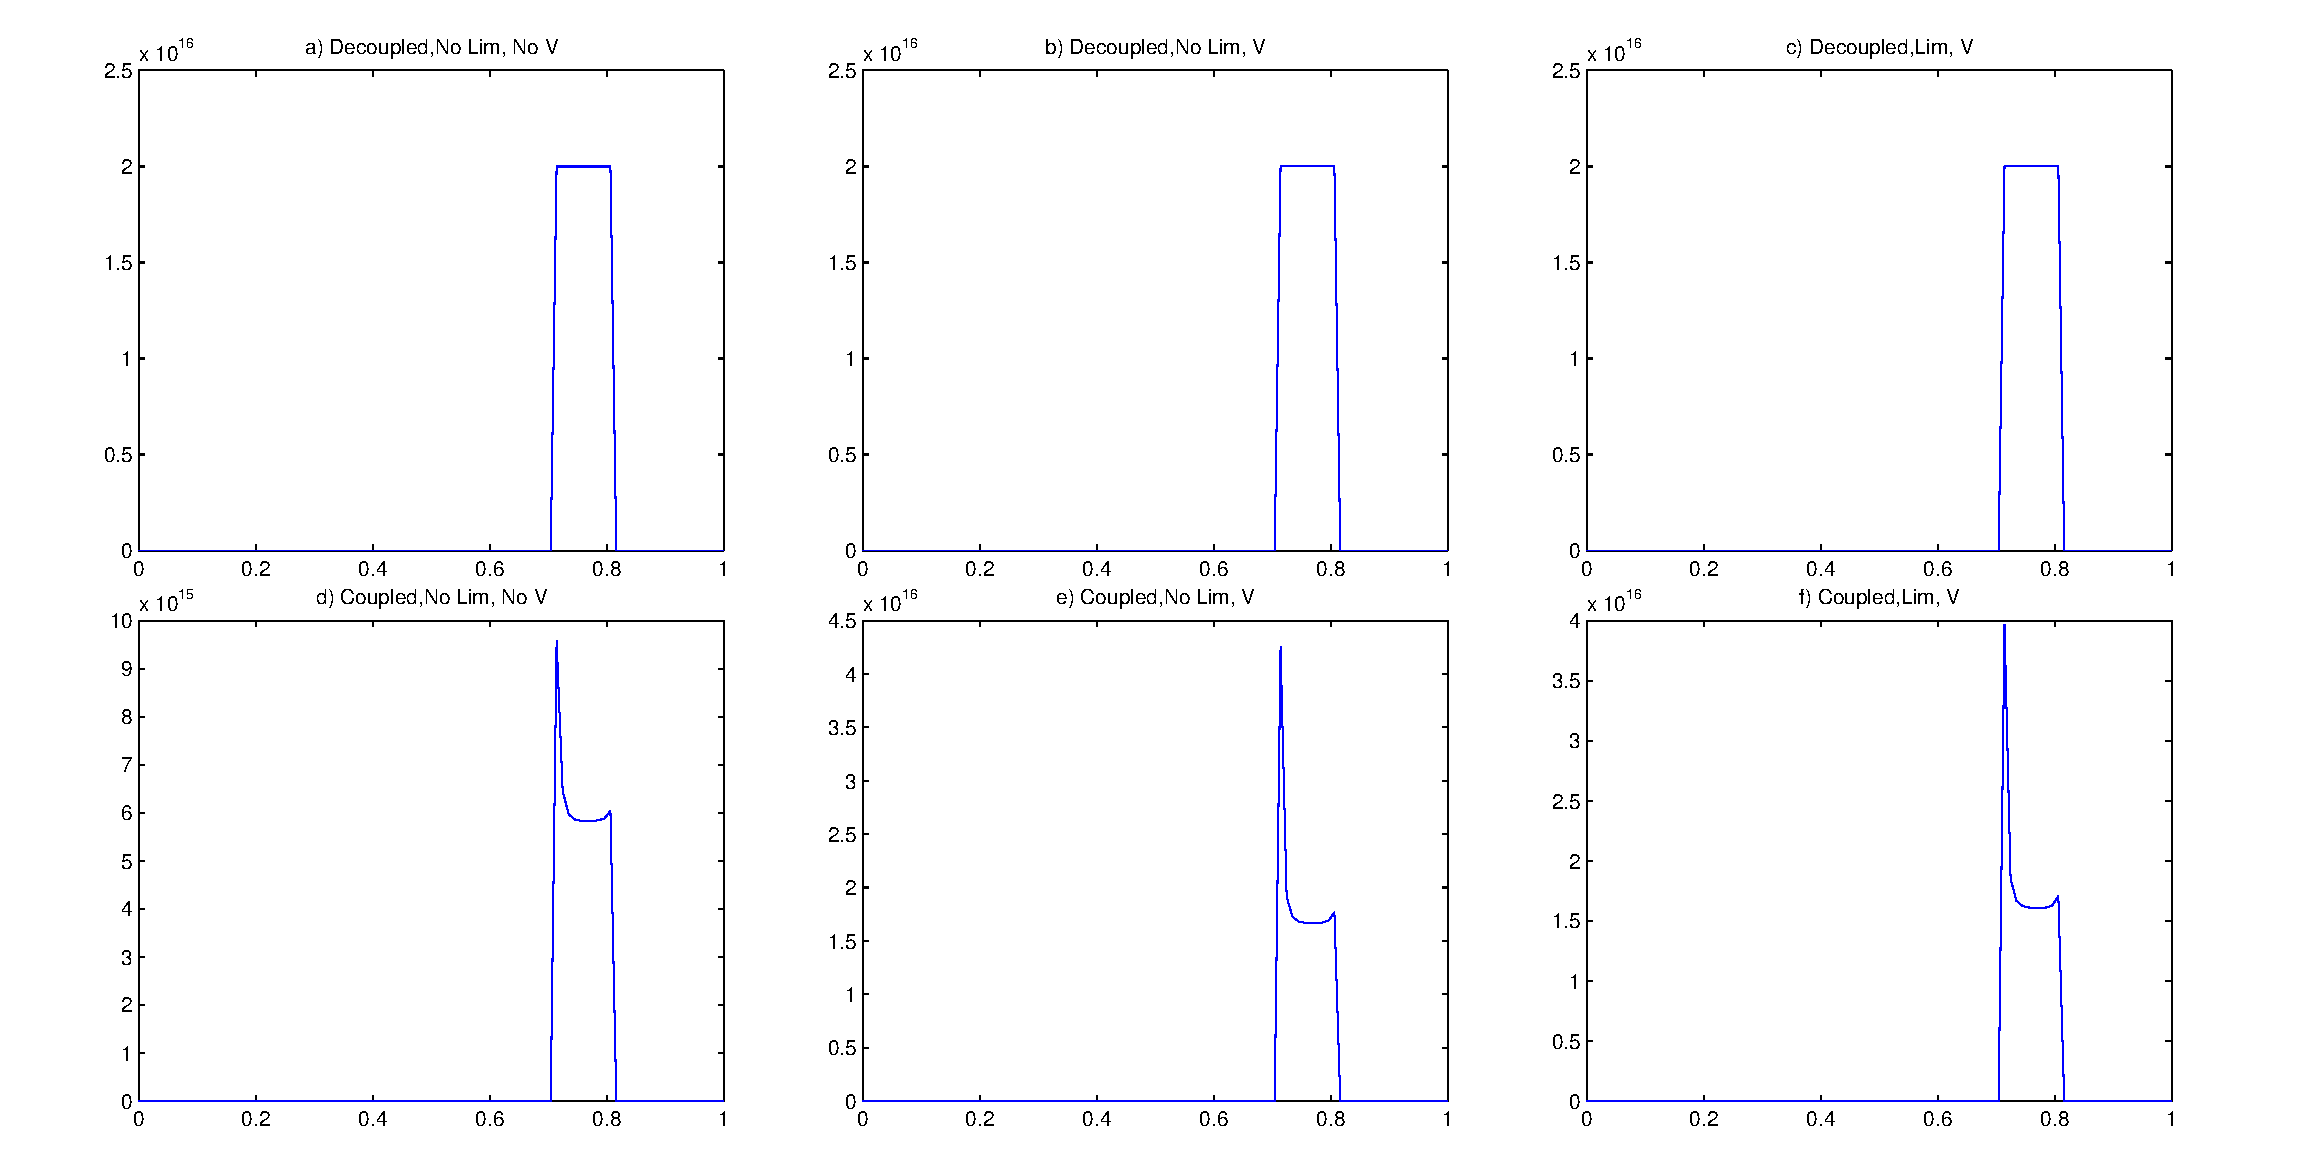
\includegraphics[scale=0.65]{p61105}
\caption{1 D Holes Horizontal} 
\end{figure}
\end{landscape}


